\documentclass[12pt,thmsa]{article}

%maths
\usepackage{amsmath}   % \sideset
\usepackage{amsthm}    % for proof
\usepackage{amsfonts}  % for \mathbb
\usepackage{mathrsfs}  % for Ralph Smith's Formal Script Font
\usepackage[mathscr]{euscript} %redefine the \mathcal command to use Euler script
\usepackage{amssymb}   % \varnothing, \bigstar, \blacksquare, \clubsuit, \blacktriangleright, \diamondsuit, \spadesuit, \dagger, \checkmark

%algorithms
\usepackage{algpseudocode}% http://ctan.org/pkg/algorithmicx
\usepackage[ruled,vlined,linesnumbered]{algorithm2e} % For algorithm
%\usepackage{algorithm}% http://ctan.org/pkg/algorithms % conflict with algorithm2e

%tables
\usepackage{booktabs}  % Allows the use of \toprule, \midrule and \bottomrule in tables
\usepackage{multirow}
\usepackage{multicol}
\usepackage{tabularx}
\usepackage[table]{xcolor} % For \cellcolor
\usepackage[export]{adjustbox}

%figures
\usepackage{graphicx}  % Allows including images
\usepackage{float}     % Force figure placement in text with [H]

%tikzpicture
\usepackage{tikz}
\usepackage{scalerel}
\usepackage{pict2e}
\usepackage{tkz-euclide}
\usetikzlibrary{matrix}
\usetikzlibrary{shapes, positioning}
\usetikzlibrary{calc}
\usetikzlibrary{patterns, arrows.meta}
\usetikzlibrary{shadows}
\usetikzlibrary{external}

%pgfplots
\usepackage{pgfplots}
\pgfplotsset{compat=newest}
\usepgfplotslibrary{statistics}
\usepgfplotslibrary{fillbetween}

%colors
\usepackage{color}     % color
\usepackage[colorinlistoftodos]{todonotes}

%other
\usepackage{cancel}
\usepackage{enumitem}
\setlist[itemize]{leftmargin=*} % global option, remove the indentation for a specific list
\usepackage{textcase}  % \MakeTextUppercase
\renewcommand{\qedsymbol}{$\blacksquare$} % change the QED symbol to a filled square
\usepackage{hyperref}
\usepackage{tocloft}

%layout
\usepackage{geometry}
\usepackage{fancyhdr}   % Fancy Headers


%------------------------------------------------------%
%              Create Center Title Page                %
%------------------------------------------------------%
\usepackage{titling}
\renewcommand\maketitlehooka{\null\mbox{}\vfill}
\renewcommand\maketitlehookd{\vfill\null}

\geometry{
	a4paper,
	total={170mm,257mm},
	left=20mm,
	right=20mm,
	top=20mm,
}

% Linhui added for newly defined color
\definecolor{forestgreen}{RGB}{34,139,34}

% Linhui added for Expectation and Variance
\newcommand{\Exp}{{\mathbb E}\! }
\newcommand{\Var}{\mbox{Var}\! }

% Linhui added for rename the command for empty set.
\let\oldemptyset\emptyset
\let\emptyset\varnothing

%------------------------------------------------------%
\makeatletter
\def\maketitle{%
	\par
	\hrule height 1.5pt\vspace{1ex}
	\par\noindent
	
	\begin{minipage}{0.5\textwidth}
		\scshape
		Purdue University $\cdot$ ece 58000 \\[1ex]
		Optimization Methods \\
		Prof. Żak
	\end{minipage}
	\begin{minipage}{0.45\textwidth}
		\raggedleft
		\MakeTextUppercase{{\@title}}\\[0.3ex] % 0.2ex height space between two line
		\textit{\@author}\\[0.2ex]
		\textit{August 1, 2022}
	\end{minipage}
	\par\vspace{1ex}
	\hrule height 1.5pt\vspace{1ex}
	\par
}
\makeatother

\author{Linhui Xie}
\title{Review of Qualify Exam}
%------------------------------------------------------%

\begin{document}
	\tableofcontents
	\newpage
	
% Part 1: Math Review
\maketitle
%------------------------------------------------------%
%------------------------------------------------------%
\section{Quadratic Forms \medskip}
%------------------------------------------------------%
%------------------------------------------------------%

%------------------------------------------------------%
\subsection{Concept}
\begin{itemize}
	\item \(f: \mathbb{R}^{n} \rightarrow \mathbb{R}\) is a \underline{quadratic} function if

	\begin{equation*}
		f(\boldsymbol{x})=\boldsymbol{x}^{T} \boldsymbol{Q} \boldsymbol{x}+\boldsymbol{b}^{T} \boldsymbol{x}+c,
	\end{equation*}
	
	where \(\boldsymbol{Q}\) is {\color{black}symmetric}.

	\item \(\boldsymbol{Q}\) is symmetric if \(\boldsymbol{Q}=\boldsymbol{Q}^{\top}\).
	
	\item A symmetric matrix \(\boldsymbol{Q}\) is said to be \underline{positive definite} (p.d.) if \(\boldsymbol{x}^{\top} \boldsymbol{Q} \boldsymbol{x}>0\) for {\color{black}all nonzero} vectors \(\boldsymbol{x}\).
	
	\item It is \underline{positive semi-definite} (p.s.d.) if \(\boldsymbol{x}^{\top} \boldsymbol{Q} \boldsymbol{x} \geq 0\) for {\color{black}all} \(\boldsymbol{x}\).
	
	\item Similarly, \underline{negative definite} (n.d.) and \underline{negative semi-definite} (n.s.d.),  if \(\boldsymbol{x}^{\top} \boldsymbol{Q} \boldsymbol{x}<0\) for {\color{black}all nonzero} vectors \(\boldsymbol{x}\), or \(\boldsymbol{x}^{\top} \boldsymbol{Q} \boldsymbol{x} \leq 0\) for {\color{black}all} \(\boldsymbol{x}\), respectively.
	
	\item If a  \(n \times n\) matrix \(\boldsymbol{Q}_{0}\) is not symmetric, we can always replace it with the symmetric, as

	\begin{equation*}
		\begin{gathered}
			\boldsymbol{Q}=\boldsymbol{Q}^{T}=\frac{1}{2}\left(\boldsymbol{Q}_{0}+\boldsymbol{Q}_{0}^{T}\right), \\
			\boldsymbol{x}^{T} \boldsymbol{Q} \boldsymbol{x}=\boldsymbol{x}^{T} \boldsymbol{Q}_{0} \boldsymbol{x}=\boldsymbol{x}^{T}\left(\frac{1}{2} \boldsymbol{Q}_{0}+\frac{1}{2} \boldsymbol{Q}_{0}^{T}\right) \boldsymbol{x}.
		\end{gathered}
	\end{equation*}
	
	\item The leading principal minors of matrix \(\boldsymbol{Q}\) are,
	
	\begin{equation*}
		\begin{gathered}
			\Delta_{1}=q_{11}, \quad \Delta_{2}=\operatorname{det}\left[\begin{array}{ll}
				q_{11} & q_{12} \\
				q_{21} & q_{22}
			\end{array}\right], 
			\Delta_{3}=\operatorname{det}\left[\begin{array}{lll}
				q_{11} & q_{12} & q_{13} \\
				q_{21} & q_{22} & q_{23} \\
				q_{31} & q_{32} & q_{33}
			\end{array}\right], \quad \ldots
		\end{gathered}
	\end{equation*}

	\item For an \(n \times n\) symmetric real matrix \(\boldsymbol{Q}\),
	\begin{equation*}
		\begin{aligned}
			\boldsymbol{Q} \text{ positive-definite }  &  \Longleftrightarrow \quad \boldsymbol{x}^{\top} \boldsymbol{Q} \boldsymbol{x}>0 \text { for all } \boldsymbol{x} \in \mathbb{R}^n \backslash\{\boldsymbol{0}\}, \\
			\boldsymbol{Q}  \text{ positive semi-definite } & \Longleftrightarrow \quad \boldsymbol{x}^{\top} \boldsymbol{Q} \boldsymbol{x} \geq 0 \text{ for all } \boldsymbol{x} \in \mathbb{R}^n, \\
			\boldsymbol{Q} \text { negative-definite } & \Longleftrightarrow \quad \boldsymbol{x}^{\top} \boldsymbol{Q} \boldsymbol{x}<0 \text { for all } \boldsymbol{x} \in \mathbb{R}^n \backslash\{\boldsymbol{0}\}, \\
			\boldsymbol{Q} \text { negative semi-definite } &\Longleftrightarrow \quad \boldsymbol{x}^{\top} \boldsymbol{Q} \boldsymbol{x} \leq 0 \text { for all } \boldsymbol{x} \in \mathbb{R}^n.
		\end{aligned}
	\end{equation*}
	
	\item For an \(n \times n\) Hermitian complex matrix \(\boldsymbol{Q}\),
	\begin{equation*}
		\begin{aligned}
			\boldsymbol{Q} \text{ positive-definite }, \boldsymbol{Q} \succ 0 &  \Longleftrightarrow \quad
			\boldsymbol{x}^{\top} \boldsymbol{Q} \boldsymbol{x}>0 \text { for all } \boldsymbol{x} \in \mathbb{C}^n \backslash\{\boldsymbol{0}\}, \\
			\boldsymbol{Q}  \text{ positive semi-definite }, \boldsymbol{Q}  \succeq 0 & \Longleftrightarrow \quad \boldsymbol{x}^{\top} \boldsymbol{Q} \boldsymbol{x} \geq 0 \text{ for all } \boldsymbol{x} \in \mathbb{C}^n, \\
			\boldsymbol{Q} \text { negative-definite }, \boldsymbol{Q}  \prec 0 & \Longleftrightarrow \quad
			\boldsymbol{x}^{\top} \boldsymbol{Q} \boldsymbol{x}<0 \text { for all } \boldsymbol{x} \in \mathbb{C}^n \backslash\{\boldsymbol{0}\}, \\
			\boldsymbol{Q} \text { negative semi-definite }, \boldsymbol{Q}  \preceq 0 &\Longleftrightarrow \quad \boldsymbol{x}^{\top} \boldsymbol{Q} \boldsymbol{x} \leq 0 \text { for all } \boldsymbol{x} \in \mathbb{C}^n.
		\end{aligned}
	\end{equation*}
	
	
	\item[\(\spadesuit\)] \(\mathscr{THEOREM}\) 3.6 Sylvester's Criterion. A quadratic form (\(\boldsymbol{Q}\) is symmetric) \(\boldsymbol{x}^{\top} \boldsymbol{Q} \boldsymbol{x}, \boldsymbol{Q}=\boldsymbol{Q}^{\top}\), is positive definite if and only if the leading principal minors of \(\boldsymbol{Q}\) are positive.

	\item[\(\spadesuit\)] \(\mathscr{THEOREM}\) 3.7  A symmetric matrix \(\boldsymbol{Q}\) is positive definite (or positive semidefinite) if and only if all eigenvalues of \(\boldsymbol{Q}\) are positive (or non-negative).

	\item A necessary condition for a real quadratic form to be positive semi-definite is that the leading principal minors be nonnegative. However, it is not a sufficient condition.
	
	\item A real quadratic form is positive semi-definite if and only if all principal minors are non-negative.
	
\end{itemize}



%------------------------------------------------------%
\subsection{Examples}
%------------------------------------------------------%
Example 1: (1) Given set \(\Omega=\left\{\boldsymbol{x} \in \mathbb{R}^{3}\right\}\),

(2) \(\Omega=\left\{\boldsymbol{x} \in \mathbb{R}^{3}: x_{1}+x_{3}=0, x_{1}+x_{2}+x_{3}=0\right\}\), is the quadratic form,

\begin{equation*}
	f(\boldsymbol{x})=\boldsymbol{x}^{\top} \boldsymbol{Q} \boldsymbol{x}=\boldsymbol{x}^{\top}\left[\begin{array}{ccc}
		5 & 3 & 0 \\
		0 & 0 & 5 \\
		7 & 3 & 1
	\end{array}\right] \boldsymbol{x},
\end{equation*}

p.d, p.s.d, n.d, n.s.d, or indefinite on \(\mathbb{R}^{3}\)?

\noindent
\textbf{Short answer:}

(1) Notice that \(\boldsymbol{Q}\) is not symmetric, first convert it to standard form

\begin{equation*}
	f(\boldsymbol{x})=\frac{1}{2} \boldsymbol{x}^{\top}\left(\boldsymbol{Q}+\boldsymbol{Q}^{\top}\right) \boldsymbol{x}=\frac{1}{2} \boldsymbol{x}^{\top}\left[\begin{array}{ccc}
		10 & 3 & 7 \\
		3 & 0 & 8 \\
		7 & 8 & 2
	\end{array}\right] \boldsymbol{x} .
\end{equation*}

Since leading principal minors \(10>0\) and \(\operatorname{det}\left[\begin{array}{cc}10 & 3 \\ 3 & 0\end{array}\right]<0, f(\boldsymbol{x})\) is indefinite on \(\mathbb{R}^{3}\).


(2) Let \(\boldsymbol{x}=\left[\begin{array}{lll}a & 0 & -a\end{array}\right]^{\top}, a \in \mathbb{R}\), and \(a \neq 0\). Then \(f(\boldsymbol{x})=-a^{2}<0\). Therefore, \(f(\boldsymbol{x})\) is negative definite on the set \(\Omega\).


%------------------------------------------------------%
\bigskip
\noindent
Example 2: Is the matrix

\begin{equation*}
	\boldsymbol{Q}=\left[\begin{array}{ccc}
		\alpha^{4} & \alpha^{3} & \alpha^{2} \\
		\alpha^{3} & \alpha^{2} & \alpha^{1} \\
		\alpha^{2} & \alpha^{1} & 1
	\end{array}\right]
\end{equation*}

where \(\alpha \in \mathbb{R}\), p.d, p.s.d, n.d, n.s.d or indefinite?

\noindent
\textbf{Short answer:}
Let \(\boldsymbol{v}=\left[\begin{array}{lll}\alpha^{2} & \alpha^{1} & 1\end{array}\right]^{\top}\). Then \(\boldsymbol{Q}=\boldsymbol{v} \boldsymbol{v}^{\top}\) and \(\boldsymbol{x}^{\top} \boldsymbol{Q} \boldsymbol{x}=\boldsymbol{x}^{\top} \boldsymbol{v} \boldsymbol{v}^{\top} \boldsymbol{x}=\left(\boldsymbol{x}^{\top} \boldsymbol{v}\right)^{2} \geq 0\). Therefore, \(\boldsymbol{Q}\) is positive semi-definite.


%------------------------------------------------------%
\bigskip
\noindent
Example 3: Find the range of the coefficient \(\beta\) for the function:

\begin{equation*}
	f\left(x_{1}, x_{2}, x_{3}\right)=2 x_{1} x_{3}-x_{1}^{2}-x_{2}^{2}-5 x_{3}^{2}-2 \beta x_{1} x_{2}-4 x_{2} x_{3}
\end{equation*}

is negative semi-definite.

\noindent
\textbf{Short answer:}
If \(f(\boldsymbol{x})\) is n.s.d, then \(-f(\boldsymbol{x})\) is p.s.d.

\begin{equation*}
	-f(\boldsymbol{x})=\boldsymbol{x}^{\top} \boldsymbol{Q} \boldsymbol{x}=\boldsymbol{x}^{\top}\left[\begin{array}{ccc}
		1 & \beta & -1 \\
		\beta & 1 & 2 \\
		-1 & 2 & 5
	\end{array}\right] \boldsymbol{x} .
\end{equation*}

Let \(\operatorname{det}\left[\begin{array}{ll}1 & \beta \\ \beta & 1\end{array}\right]=1-\beta^{2} \geq 0\) and \(\operatorname{det}(\boldsymbol{Q})=-5 \beta^{2}-4 \beta \geq 0\), we have \(\beta \in\left[-\frac{4}{5}, 0\right]\).

\bigskip

\noindent
[Ref]: Edwin K.P. Chong, Stanislaw H. Żak, ``PART I MATHEMATICAL REVIEW" in ``An introduction to optimization", 4th Edition, John Wiley and Sons, Inc. 2013.

%%------------------------------------------------------%
%------------------------------------------------------%
\section{Gradient and Hessian}
%------------------------------------------------------%
%------------------------------------------------------%

%------------------------------------------------------%
\subsection{Concept}
\begin{itemize}
	\item[({\bf{1}})] Given \(f: \mathbb{R} \rightarrow \mathbb{R}\), if the limit exists, the derivative of \(f\) is a function \(f^{\prime}: \mathbb{R} \rightarrow \mathbb{R}\) given by
	\[
	D_{x}(f(x)) = \frac{\mathrm{d} f}{\mathrm{d} x} = f^{\prime}(x)=\lim _{h \rightarrow 0} \frac{f(x+h)-f(x)}{h}.
	\]
	
	\item[({\bf{2}})] Given \(f: \mathbb{R}^{n} \rightarrow \mathbb{R}\), consider a scalar \( f(\boldsymbol{x}) = a_{1} x_{1}+a_{2} x_{2}+\cdots+a_{n} x_{n} =  \boldsymbol{a}^{\top} \boldsymbol{x}\).
	
	For \textbf{derivative} rule (2), 
	\[ 
	{\color{red}{D_{\boldsymbol{x}}}} { f(\boldsymbol{x}) } =
	{\color{black}{D(}}{ \boldsymbol{a}^{\top} \boldsymbol{x} }{\color{black})} 
	= 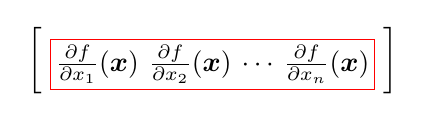
\begin{tikzpicture}[baseline=(current bounding box.center)]
		\matrix (m) [matrix of math nodes, inner sep=1.8pt, row sep=0pt, left delimiter={[},right delimiter={]}] {
			\frac{\partial f}{\partial x_1} (\boldsymbol{x}) & \frac{\partial f}{\partial x_2}(\boldsymbol{x}) & \cdots & \frac{\partial f}{\partial x_n}(\boldsymbol{x}) \\
		};
		\draw[red] (m-1-1.north west) rectangle (m-1-4.south east);
	\end{tikzpicture}
	=\left[\begin{array}{cccc}
		a_{1} & a_{2} &  \cdots & a_{n}
	\end{array}
	\right] = {\color{red}{ \boldsymbol{a}^{\top} }}.
	\]
	
	For \textbf{gradient} rule (2), \underline{if \(f: \mathbb{R}^{n} \rightarrow \mathbb{R}\) is differentiable}, then the \textit{gradient} of \(f\) is a function \(\nabla f: \mathbb{R}^{n} \rightarrow \mathbb{R}^{n}\) given by
	\[  {\color{blue}{\nabla}_{\boldsymbol{x}} } f(\boldsymbol{x})
	= 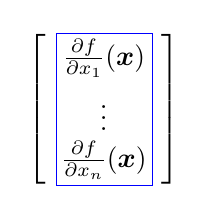
\begin{tikzpicture}[baseline=(current bounding box.center)]
		\matrix (m) [matrix of math nodes, inner sep=2pt, left delimiter={[},right delimiter={]}, nodes in empty cells] {
			\frac{\partial f}{\partial x_1} (\boldsymbol{x}) \\
			|[minimum height=0.5cm]|  \vdots \\
			\frac{\partial f}{\partial x_n} (\boldsymbol{x}) \\
		};
		\draw[blue] (m-1-1.north west) rectangle (m-3-1.south east);
	\end{tikzpicture}
	= \left[ \begin{array}{c} a_1  \\ \vdots \\ a_n \end{array} \right]
	= {\color{blue}{ \boldsymbol{a} }}
	= D_{\boldsymbol{x}} f(\boldsymbol{x}) ^{\top}.
	\] 
	
	\item[({\bf{3}})] Given \(\boldsymbol{g}: \mathbb{R} \rightarrow \mathbb{R}^m \), here \(t \in \mathbb{R} \) is a scalar. \(\boldsymbol{g}(t)\) is a column vector.
	\[
	\begin{aligned}
		\boldsymbol{g}(t) =
		\left[
		\begin{array}{c}
			g_{1}(t) \\
			\vdots \\
			g_{m}(t)
		\end{array}
		\right], \quad
		D_{t} \boldsymbol{g}(t) & =\left[
		\begin{aligned}
			\frac{\mathrm{d}}{\mathrm{d} t}g_{1}(t) \\
			\vdots \qquad \\
			\frac{\mathrm{d}}{\mathrm{d} t}g_{m}(t)
		\end{aligned}
		\right] =\left[\begin{array}{c}
			g_{1}^{\prime}(t) \\
			\vdots \\
			g_{m}^{\prime}(t)
		\end{array}\right].  \\
	\end{aligned}
	\]
	
	\item[({\bf{4}})] Consider \(\boldsymbol{g}: \mathbb{R}^{n} \rightarrow \mathbb{R}^m \),  here \( \boldsymbol{x} \in  \mathbb{R}^n \) is a vector. Since \(g_{i}(\boldsymbol{x})\) is a scalar, \(\boldsymbol{g}=\left[g_1, \ldots, g_m\right]^{\top} \), \(\boldsymbol{g}(\boldsymbol{x})\) is a column vector.
	\[
	\begin{aligned}
		\boldsymbol{g} \left( \boldsymbol{x} \right)=
		\left[
		\begin{array}{c}
			g_{1}( \boldsymbol{x} ) \\
			g_{2}( \boldsymbol{x} ) \\
			\vdots \\
			g_{m}( \boldsymbol{x} )
		\end{array}
		\right], 
		D_{\boldsymbol{x}} \boldsymbol{g}\left( \boldsymbol{x} \right) & =\left[
		\begin{array}{c}
			{ \color{red}D_{\boldsymbol{x}} } g_{1}\left( x_1,x_2,\cdots,x_n \right) \vspace{0.3cm} \\
			{ \color{red}D_{\boldsymbol{x}} } g_{2}\left( x_1,x_2,\cdots,x_n \right)  \\
			\vdots \\
			{ \color{red}D_{\boldsymbol{x}} } g_{m}\left( x_1,x_2,\cdots,x_n \right) 
		\end{array}
		\right]
		= 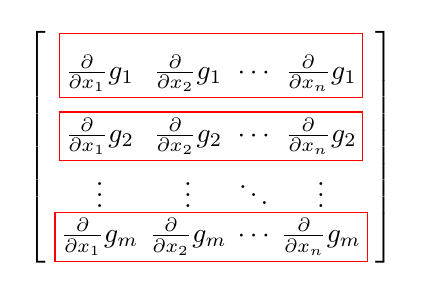
\begin{tikzpicture}[baseline=(current bounding box.center)]
			\matrix [matrix of math nodes, inner sep=2pt, left delimiter={[},right delimiter={]}] (m) {
				|[minimum height=1cm]| \frac{\partial}{\partial x_1} g_1 & \frac{\partial}{\partial x_2} g_1 & \cdots & \frac{\partial}{\partial x_n} g_1 \\
				\frac{\partial}{\partial x_1} g_2 & \frac{\partial}{\partial x_2} g_2 & \cdots & \frac{\partial}{\partial x_n} g_2 \\
				\vdots & \vdots & \ddots & \vdots \\
				\frac{\partial}{\partial x_1} g_m & \frac{\partial}{\partial x_2} g_m & \cdots & \frac{\partial}{\partial x_n} g_m \\
			};
			\draw[red] (m-1-1.north west) rectangle (m-1-4.south east);
			\draw[red] (m-2-1.north west) rectangle (m-2-4.south east);
			\draw[red] (m-4-1.north west) rectangle (m-4-4.south east);
		\end{tikzpicture}
		= \mathbf{J}.
	\end{aligned}
	\]
	The matrix \(\mathbf{J}\) is called the \underline{Jacobian matrix}, or derivative matrix, of function \(\boldsymbol{g}\).
	
	\item Note that, \( D \left( f(\boldsymbol{x}) \right)\) is spreading the derivative of the polynomials on the horizontal direction. The second derivative of \(f: \mathbb{R}^{n} \rightarrow \mathbb{R}\) (also called the Hessian of \(f\) ) is
	\[ D^{2} \left( f(\boldsymbol{x}) \right)
	= D \left(  D f \left( \boldsymbol{x} \right)^{\top} \right)
	= D(\nabla f(\boldsymbol{x}))
	= \left[\begin{array}{c}    
		D\left(\frac{\partial f}{ \color{forestgreen}{\partial x_{1}} }\right) \\    
		D\left(\frac{\partial f}{ \color{forestgreen}{\partial x_{2}} }\right) \\    
		\vdots \\    
		D\left(\frac{\partial f}{ \color{forestgreen}{\partial x_{n}} }\right)    
	\end{array}
	\right]
	=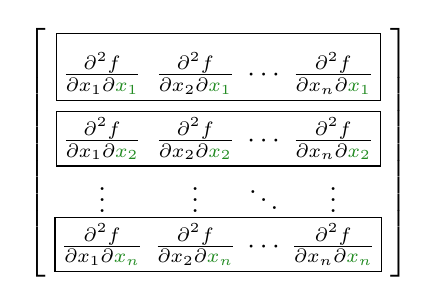
\begin{tikzpicture}[baseline=(current bounding box.center)]
		\matrix (m) [matrix of math nodes, inner sep=2pt, left delimiter={[}, right delimiter={]}] {
			|[minimum height=1cm]| \frac{\partial^2 f}{\partial x_1 \partial \textcolor{forestgreen}{x_1}} & \frac{\partial^2 f}{\partial x_2 \partial \textcolor{forestgreen}{x_1}} & \cdots & \frac{\partial^2 f}{\partial x_n \partial \textcolor{forestgreen}{x_1}} \\
			\frac{\partial^2 f}{\partial x_1 \partial \textcolor{forestgreen}{x_2}} & \frac{\partial^2 f}{\partial x_2 \partial \textcolor{forestgreen}{x_2}} & \cdots & \frac{\partial^2 f}{\partial x_n \partial \textcolor{forestgreen}{x_2}} \\
			\vdots & \vdots & \ddots & \vdots \\
			\frac{\partial^2 f}{\partial x_1 \partial \textcolor{forestgreen}{x_n}} & \frac{\partial^2 f}{\partial x_2 \partial \textcolor{forestgreen}{x_n}} & \cdots & \frac{\partial^2 f}{\partial x_n \partial \textcolor{forestgreen}{x_n}} \\
		};
		\foreach \i in {1,2,4} {
			\draw (m-\i-1.north west) rectangle (m-\i-4.south east);
		}
	\end{tikzpicture} .
	\]
\end{itemize}

\begin{itemize}
	\item In summary, the derivative rules are listed as,
	% align automatically places the equations in math mode 
	\begin{align*}
		{\color{red} D(} \boldsymbol{a}^{\top} \boldsymbol{x} {\color{red})} 
		&= \boldsymbol{a}^{\top}, \qquad &
		\fbox{\parbox{0.36\textwidth}{\( (2) f: \mathbb{R}^{n} \rightarrow \mathbb{R}, f(\boldsymbol{x}) =  \boldsymbol{a}^{\top} \boldsymbol{x} \)}} \\
		{\color{red} D(} \boldsymbol{g}(t) {\color{red})} 
		&= \left[ \begin{array}{c} \vdots \\ g_{*}'(t) \\ \vdots \end{array} \right], \qquad &
		\fbox{\parbox{0.36\textwidth}{\( (3) \boldsymbol{g}: \mathbb{R} \rightarrow \mathbb{R}^{n}, \boldsymbol{g}(t) =  \left[ \begin{array}{c} \vdots \\ g_{*}(t) \\ \vdots \end{array} \right] \)}} \\
		{\color{red} D(} \mathbf{A} \boldsymbol{x} {\color{red})} 
		&= {\color{black} \mathbf{A}}, \qquad &
		\fbox{\parbox{0.36\textwidth}{\( (4) \boldsymbol{g}: \mathbb{R}^{n} \rightarrow \mathbb{R}^{m}, \boldsymbol{g}(\boldsymbol{x}) =  \mathbf{A} \boldsymbol{x} \)}} \\
		{\color{red} D(} \mathbf{A}(\alpha \boldsymbol{x}) {\color{red})} 
		&= {\color{black} \alpha \mathbf{A}}, \\
		\frac{\mathrm{d}}{\mathrm{d} \alpha}( {\color{black}\mathbf{A}(\alpha \boldsymbol{x})} ) &= {\color{black} \mathbf{A} \boldsymbol{x}}, \\
		{\color{blue}\nabla} \boldsymbol{a}^{\top} \boldsymbol{x} 
		&= \boldsymbol{a},  \qquad & 
		\fbox{\parbox{0.36\textwidth}{\( (2) f: \mathbb{R}^{n} \rightarrow \mathbb{R}, f(\boldsymbol{x}) =  \boldsymbol{a}^{\top} \boldsymbol{x} \)}} \\
		{\color{blue}\nabla} \mathbf{A} \boldsymbol{x} 
		&= \mathbf{A}^{\top}, \qquad & 
		\fbox{\parbox{0.36\textwidth}{\( (4) \boldsymbol{g}: \mathbb{R}^{n} \rightarrow \mathbb{R}^{m}, \boldsymbol{g}(\boldsymbol{x}) =  \mathbf{A} \boldsymbol{x} \)}} \\
		{\color{blue}\nabla} \mathbf{A}(\alpha \boldsymbol{x}) 
		&=  \alpha \mathbf{A}^{\top}. \\
	\end{align*}

	\item Note that for \underline{ \(f: \mathbb{R}^n \rightarrow \mathbb{R}\) }, we have
	\[
	{\color{blue} \nabla} f(\boldsymbol{x})={\color{red} D} f(\boldsymbol{x})^{\top}.
	\]
\end{itemize}

%------------------------------------------------------%
\subsection{Differentiation product rules}
\textbf{i)} Let \(f: \mathbb{R} \rightarrow \mathbb{R}\) and \(g: \mathbb{R} \rightarrow \mathbb{R}\) be two differentiable functions, \(x \in \mathbb{R}\),
\[ 
\begin{aligned}
	D \bigg (f(x) g(x) \bigg )
	& = f(x)  D g(x)
	+g(x)  D f(x),  \\
	\nabla \bigg (f(x) g(x) \bigg )
	& = f(x)  \nabla g(x)
	+g(x)  \nabla f(x). 
\end{aligned}
\]

\noindent
\textbf{ii)} Let \(f: \mathbb{R}^{n} \rightarrow \mathbb{R}\) and \(g: \mathbb{R}^{n} \rightarrow \mathbb{R}\) be two differentiable functions, \(\boldsymbol{x} \in \mathbb{R}^{n}\),
\[ 
\begin{aligned}
	D \bigg (f(\boldsymbol{x}) g(\boldsymbol{x}) \bigg )
	& = f(\boldsymbol{x}) \big [\begin{array}{ccc}
		&D g(\boldsymbol{x}) & \end{array} \big ] 
	+g(\boldsymbol{x}) \big [\begin{array}{ccc} & D f(\boldsymbol{x}) &
	\end{array} \big ], \\
	\nabla \bigg (f(\boldsymbol{x}) g(\boldsymbol{x}) \bigg )
	& = f(\boldsymbol{x}) \left [\begin{array}{c}
		\\ \nabla g(\boldsymbol{x}) \\  \\ \end{array} \right ] 
	+g(\boldsymbol{x}) \left [\begin{array}{c} \\ \nabla f(\boldsymbol{x}) \\ \\
	\end{array} \right ].
\end{aligned}
\]

\noindent
\textbf{iii)} Let \( \boldsymbol{f}: \mathbb{R}^{n} \rightarrow \mathbb{R}^{m}\) and \( \boldsymbol{g}: \mathbb{R}^{n} \rightarrow \mathbb{R}^{m}\) be two differentiable functions, \(\boldsymbol{x} \in \mathbb{R}^{n}\),
\[ 
\begin{aligned}
	D \bigg (\boldsymbol{f}(\boldsymbol{x})^{\top} \boldsymbol{g}(\boldsymbol{x}) \bigg )
	& =\boldsymbol{f}(\boldsymbol{x})^{\top} D \boldsymbol{g}(\boldsymbol{x})+\boldsymbol{g}(\boldsymbol{x})^{\top} D \boldsymbol{f}(\boldsymbol{x}), \\
	\nabla \bigg (\boldsymbol{f}(\boldsymbol{x})^{\top} \boldsymbol{g}(\boldsymbol{x}) \bigg )
	& =\boldsymbol{f}(\boldsymbol{x})^{\top} \nabla \boldsymbol{g}(\boldsymbol{x})+\boldsymbol{g}(\boldsymbol{x})^{\top} \nabla \boldsymbol{f}(\boldsymbol{x}). \\
\end{aligned}
\]

\begin{itemize}
	\item Based on the above \textbf{derivative} rule, we have
	
	\textbf{1.} Consider \(\mathbf{A} \in \mathbb{R}^{m \times n}\) be a given matrix and \(\boldsymbol{y} \in \mathbb{R}^{m}\) a given vector. Then,
	\begin{align*}
		D\left(\boldsymbol{y}^{\top} \mathbf{A} \boldsymbol{x}\right) &=
		\boldsymbol{y}^{\top} \mathbf{A}, \\
		D\left(\boldsymbol{x}^{\top} \mathbf{A} \boldsymbol{x}\right) &=
		\boldsymbol{x}^{\top}\left(\mathbf{A}+\mathbf{A}^{\top}\right).  \qquad
		\fbox{\parbox{0.1\textwidth}{ if \(m=n\) }}
	\end{align*}
	
	
	\textbf{2.} Consider \(\mathbf{A} \in \mathbb{R}^{m \times n}\) be a given matrix and \(\boldsymbol{y} \in \mathbb{R}^{n}\) a given vector. Then,
	\[ D\left(\boldsymbol{y}^{\top} \boldsymbol{x}\right)=\boldsymbol{y}^{\top}. \]
	
	\textbf{3.} Consider if \(\mathbf{Q}\) is a symmetric matrix, then
	\[
	D\left(\boldsymbol{x}^{\top} \mathbf{Q} \boldsymbol{x}\right)=2 \boldsymbol{x}^{\top} \mathbf{Q}.
	\]
	
	In particular,
	\[
	D\left(\boldsymbol{x}^{\top} \boldsymbol{x}\right)=2 \boldsymbol{x}^{\top}.
	\]
	
	\item Based on the above \textbf{gradient} rule, we have
	
	\textbf{1.} Consider \(\mathbf{A} \in \mathbb{R}^{m \times n}\) be a given matrix and \(\boldsymbol{y} \in \mathbb{R}^{m}\) a given vector. Then,
	\begin{align*}
		\nabla \left(\boldsymbol{y}^{\top} \mathbf{A} \boldsymbol{x}\right) &= \mathbf{A}^{\top} \boldsymbol{y}, \\
		\nabla  \left(\boldsymbol{x}^{\top} \mathbf{A} \boldsymbol{x}\right) &=
		\left(\mathbf{A}+\mathbf{A}^{\top}\right) \boldsymbol{x}.  \qquad
		\fbox{\parbox{0.1\textwidth}{ if \(m=n\) }}
	\end{align*}
	
	
	\textbf{2.} Consider \(\mathbf{A} \in \mathbb{R}^{m \times n}\) be a given matrix and \(\boldsymbol{y} \in \mathbb{R}^{n}\) a given vector. Then,
	\[ \nabla \left(\boldsymbol{y}^{\top} \boldsymbol{x}\right)=\boldsymbol{y}. \]
	
	\textbf{3.} Consider if \(\mathbf{Q}\) is a symmetric matrix, then
	\[
	\nabla \left(\boldsymbol{x}^{\top} \mathbf{Q} \boldsymbol{x}\right)=2  \mathbf{Q} \boldsymbol{x}.
	\]
	
	In particular,
	\[
	\nabla \left(\boldsymbol{x}^{\top} \boldsymbol{x}\right)=2 \boldsymbol{x}.
	\]
	
\end{itemize}

%------------------------------------------------------%
\subsection{Examples}
%------------------------------------------------------%
Example 1: For the function

\begin{equation*}
	f(\boldsymbol{x})=\boldsymbol{x}^{\top} \boldsymbol{Q} \boldsymbol{x}=\boldsymbol{x}^{\top}\left[\begin{array}{cccc}
		1 & 0 & 0 & 8 \\
		8 & 0 & 1 & 0 \\
		0 & 1 & 0 & 5 \\
		8 & 0 & 3 & 1
	\end{array}\right] \boldsymbol{x}
\end{equation*}

find \(D f(\boldsymbol{x})\) and \(F(\boldsymbol{x})\).

\noindent
\textbf{Short answer:}

\begin{equation*}
	\begin{aligned}
		f(\boldsymbol{x}) & =\frac{1}{2} \boldsymbol{x}^{\top}\left(\boldsymbol{Q}+\boldsymbol{Q}^{\top}\right)\boldsymbol{x} \\
		& =\frac{1}{2} \boldsymbol{x}^{\top}\left[\begin{array}{cccc}
			2 & 8 & 0 & 16 \\
			8 & 0 & 2 & 0 \\
			0 & 2 & 0 & 8 \\
			16 & 0 & 8 & 2
		\end{array}\right] \boldsymbol{x} \\
		& = \frac{1}{2} \boldsymbol{x}^{\top} \tilde{\boldsymbol{Q}} \boldsymbol{x} .
	\end{aligned}
\end{equation*}

Therefore, \(D f(\boldsymbol{x})=\boldsymbol{x}^{\top} \tilde{\boldsymbol{Q}}\), and \(F(\boldsymbol{x})=\tilde{\boldsymbol{Q}}\).

%------------------------------------------------------%
\bigskip
\noindent
Example 2: Find \(D f(\boldsymbol{x})\) of \(f(\boldsymbol{x})=\boldsymbol{x}^{\top}\left[\begin{array}{ll}1 & 5 \\ 2 & 3\end{array}\right] \boldsymbol{x}-\boldsymbol{x}^{\top}\left[\begin{array}{c}-2 \\ 3\end{array}\right]+\pi\); Find the Hessian of \(f(\boldsymbol{x})=\frac{1}{2} \boldsymbol{x}^{\top}\left[\begin{array}{ll}2 & 3 \\ 7 & 1\end{array}\right] \boldsymbol{x}-\boldsymbol{x}^{\top}\left[\begin{array}{c}1 \\ -3\end{array}\right]+\log 3\).

\noindent
\textbf{Short answer:}

(1) \(f(\boldsymbol{x})=\frac{1}{2} \boldsymbol{x}^{\top}\left[\begin{array}{ll}2 & 7 \\ 7 & 6\end{array}\right] \boldsymbol{x}-\left[\begin{array}{ll}-2 & 3\end{array}\right] \boldsymbol{x}+\pi\). Therefore,

\begin{equation*}
	\begin{aligned}
		D f(\boldsymbol{x}) & =\boldsymbol{x}^{\top}\left[\begin{array}{ll}
			2 & 7 \\
			7 & 6
		\end{array}\right]-\left[\begin{array}{ll}
			-2 & 3
		\end{array}\right] \\
		& =\left[2 \boldsymbol{x}_{1}+7 \boldsymbol{x}_{2}+2 \quad 7 \boldsymbol{x}_{1}+6 \boldsymbol{x}_{2}-3\right] .
	\end{aligned}
\end{equation*}

(2) \(F(\boldsymbol{x})=\left[\begin{array}{ll}2 & 5 \\ 5 & 1\end{array}\right]\)

%------------------------------------------------------%
\bigskip
\noindent
Example 3: For the function \(f=f\left(x_{1}, x_{2}\right)=x_{1}^{2} x_{2}+x_{2}^{3} x_{1}\),

(1) find the gradient of \(f\) at \(\boldsymbol{x}=\left[\begin{array}{ll}2 & 1\end{array}\right]^{\top}\);

(2) find the rate of increase of \(f\) at the point \(\boldsymbol{x}=\left[\begin{array}{ll}2 & 1\end{array}\right]^{\top}\) in the direction \(\boldsymbol{d}=\left[\begin{array}{ll}4 & 3\end{array}\right]^{\top}\).

\noindent
\textbf{Short answer:}
(1) \(\nabla f(\boldsymbol{x})=\left[\begin{array}{l}\frac{\partial f}{\partial x_{1}} \\ \frac{\partial f}{\partial x_{2}}\end{array}\right]=\left[\begin{array}{l}2 x_{1} x_{2}+x_{2}^{3} \\ x_{1}^{2}+3 x_{1} x_{2}^{2}\end{array}\right], \nabla f(\left[\begin{array}{c}2 \\ 1\end{array}\right])=\left[\begin{array}{c}5 \\ 10\end{array}\right]\).

(2) \(\frac{\boldsymbol{d}^{\top}}{\|\boldsymbol{d}\|} \nabla f(\boldsymbol{x})=10\).


%------------------------------------------------------%
\bigskip
\noindent
Example 4: Consider the function

\begin{equation*}
	f(\boldsymbol{x})=\left(\boldsymbol{a}^{\top} \boldsymbol{x}\right)\left(\boldsymbol{b}^{\top} \boldsymbol{x}\right),
\end{equation*}

where \(\boldsymbol{a}, \boldsymbol{b}\), and \(\boldsymbol{x}\) are \(n\)-dimensional vectors.

(1) Find \(\nabla f(\boldsymbol{x})\).

(2) Find the Hessian \(F(\boldsymbol{x})\).

\noindent
\textbf{Short answer:}
(1) We have

\begin{equation*}
	f(\boldsymbol{x})=\left(\boldsymbol{a}^{\top} \boldsymbol{x}\right)\left(\boldsymbol{b}^{\top} \boldsymbol{x}\right)=\boldsymbol{x}^{\top}\left(\boldsymbol{a} \boldsymbol{b}^{\top}\right) \boldsymbol{x}=\boldsymbol{x}^{\top} \boldsymbol{Q} \boldsymbol{x},
\end{equation*}

where \(\boldsymbol{Q} \in \mathbb{R}^{n \times n}\). Note that \(\boldsymbol{Q}\) can be non-symmetric. We then first symmetrize the quadratic form as

\begin{equation*}
	f=\frac{1}{2} \boldsymbol{x}^{\top}\left(\boldsymbol{Q}+\boldsymbol{Q}^{\top}\right) \boldsymbol{x}=\frac{1}{2} \boldsymbol{x}^{\top}\left(\boldsymbol{a} \boldsymbol{b}^{\top}+\boldsymbol{b} \boldsymbol{a}^{\top}\right) \boldsymbol{x} .
\end{equation*}

Therefore,

\begin{equation*}
	\nabla f(\boldsymbol{x})=\left(\boldsymbol{a} \boldsymbol{b}^{\top}+\boldsymbol{b} \boldsymbol{a}^{\top}\right) \boldsymbol{x}
\end{equation*}

(2) \(F(x)=\boldsymbol{a} \boldsymbol{b}^{\top}+\boldsymbol{b} \boldsymbol{a}^{\top}\).

\bigskip

\noindent
[Ref]: Edwin K.P. Chong, Stanislaw H. Żak, ``PART I MATHEMATICAL REVIEW" in ``An introduction to optimization", 4th Edition, John Wiley and Sons, Inc. 2013.

%%------------------------------------------------------%
%------------------------------------------------------%
\section{Direction of Maximum Increase}
%------------------------------------------------------%
%------------------------------------------------------%

\subsection{Concept}
\begin{itemize}
	\item A vector \(\boldsymbol{d} \in \mathbb{R}^{n}, \boldsymbol{d} \neq \boldsymbol{0}\), is a feasible direction at \( \boldsymbol{x} \in \Omega\) if there exists \(\alpha_{0}>0\) such that \(\boldsymbol{x}+\alpha \boldsymbol{d} \in \Omega\) for all \( \alpha \in\left[0, \alpha_{0}\right] \).

	\item Let \(f: \mathbb{R}^{n} \rightarrow \mathbb{R}\) be a real-valued function and let \(\boldsymbol{d}\) be a feasible direction at \(\boldsymbol{x} \in \Omega \). The directional derivative of \(f\) in the direction \(\boldsymbol{d}\), denoted \(\partial f / \partial \boldsymbol{d}\) is the real-valued function defined by
	
	\[
	\frac{\partial f}{\partial \boldsymbol{d}}(\boldsymbol{x})=\lim _{\alpha \rightarrow 0} \frac{f(\boldsymbol{x}+\alpha \boldsymbol{d})-f(x)}{\alpha} = \boldsymbol{d}^{\top} \nabla f(\boldsymbol{x})
	= \sum_{i=1}^{n} \frac{\partial f(\boldsymbol{x})}{x_i} d_i
	\]

	\item If Euclidean norm \(\|\boldsymbol{d}\|_2=1\), then \(\partial f / \partial \boldsymbol{d}\) is the \underline{rate of increase} of \(f\) at \(\boldsymbol{x}\) in the direction \(\boldsymbol{d}\).
	
	\[\frac{\partial f}{\partial \boldsymbol{d}}(\boldsymbol{x})=\left.\frac{d}{d \alpha} f(\boldsymbol{x}+\alpha \boldsymbol{d})\right|_{\alpha=0}=\nabla f(\boldsymbol{x})^{\top} \boldsymbol{d}=\langle\nabla f(\boldsymbol{x}), \boldsymbol{d}\rangle=\boldsymbol{d}^{\top} \nabla f(\boldsymbol{x}) \]

	\item If Euclidean norm \(\|\boldsymbol{d}\|_2 \neq 1\), the rate of increase of \(f\) at \(\boldsymbol{x}\) in the direction \(\boldsymbol{d}\), normalize \(\boldsymbol{d}\), replace \(\boldsymbol{d}\) with \(\frac{\boldsymbol{d}}{\|\boldsymbol{d}\|_2}\), that is, \(\frac{\boldsymbol{d}^{\top}}{\|\boldsymbol{d}\|_2} \nabla f(\boldsymbol{x}) \).
	
	\[ \left\| \frac{\boldsymbol{d}}{\|\boldsymbol{d}\|} \right\| 
	= \left\| \frac{1}{\|\boldsymbol{d}\|}  \left[ \begin{array}{c} \\ \boldsymbol{d} \\ \\ \end{array} \right]\right \|
	= \frac{1}{\|\boldsymbol{d}\|}  \|\boldsymbol{d}\|
	= 1 \]
\end{itemize}

%------------------------------------------------------%
\subsection{Practice problems}
\begin{enumerate}
	\item Given the following function,
\end{enumerate}

\begin{equation*}
	f\left(x_{1}, x_{2}\right)=x_{1}^{2} x_{2}+x_{2}^{3} x_{1} .
\end{equation*}

(1) In what direction does the function \(f\) increase most rapidly at the point \(\boldsymbol{x}^{(0)}=\left[\begin{array}{ll}2 & 1\end{array}\right]^{\top}\) ?

(2) What is the rate of increase of \(f\) at the point \(\boldsymbol{x}^{(0)}\) in the direction of maximum increase of \(f\) ?

(3) Find the rate of increase of \(f\) at the point \(\boldsymbol{x}^{(0)}\) in the direction \(\boldsymbol{d}=\left[\begin{array}{ll}4 & 3\end{array}\right]^{\top}\).

\textbf{Short answer:}
(1) A differentiable function \(f\) increases most rapidly in the direction of the gradient. In this problem, we have

\begin{equation*}
	\nabla f(\boldsymbol{x})=\left[\begin{array}{l}
		2 x_{1} x_{2}+x_{2}^{3} \\
		x_{1}^{2}+3 x_{1} x_{2}^{2}
	\end{array}\right] .
\end{equation*}

Hence,

\begin{equation*}
	\nabla f\left(\boldsymbol{x}^{(0)}\right)=\left[\begin{array}{c}
		5 \\
		10
	\end{array}\right]
\end{equation*}

(2) The rate of increase of \(f\) at \(\boldsymbol{x}^{(0)}\) in the direction \(\nabla f\left(\boldsymbol{x}^{(0)}\right)\) is

\begin{equation*}
	\nabla f\left(\boldsymbol{x}^{(0)}\right)^{\top} \frac{\nabla f\left(\boldsymbol{x}^{(0)}\right)}{\left\|\nabla f\left(\boldsymbol{x}^{(0)}\right)\right\|}=\left\|\nabla f\left(\boldsymbol{x}^{(0)}\right)\right\|=5 \sqrt{5} .
\end{equation*}

(3) The rate of increase of \(f\) at \(\boldsymbol{x}^{(0)}\) in the direction \(\boldsymbol{d}\) is

\begin{equation*}
	\nabla f\left(\boldsymbol{x}^{(0)}\right)^{\top} \frac{\boldsymbol{d}}{\|\boldsymbol{d}\|}=\left[\begin{array}{ll}
		5 & 10
	\end{array}\right]\left[\begin{array}{l}
		4 \\
		3
	\end{array}\right] \frac{1}{5}=10 .
\end{equation*}

%------------------------------------------------------%
\bigskip
\noindent
\begin{enumerate}
	\setcounter{enumi}{1}
	\item Find the range of values of the parameter \(a\) for which \(\boldsymbol{d}=\left[\begin{array}{ll}a & 1\end{array}\right]^{\top}\) is a direction of ascent of
\end{enumerate}

\begin{equation*}
	f=f\left(x_{1}, x_{2}\right)=x_{1}^{3}+x_{1} x_{2}-x_{1}^{2} x_{2}^{2},
\end{equation*}

at the point \(\boldsymbol{x}^{(0)}=\left[\begin{array}{ll}1 & 1\end{array}\right]^{\top}\).


\textbf{Short answer:}
For the direction of ascent, we have \(\boldsymbol{d}^{\top} \nabla f>0\). We first calculate the gradient

\begin{equation*}
	\nabla f(\boldsymbol{x})=\left[\begin{array}{c}
		3 x_{1}^{2}+x_{2}-2 x_{1} x_{2}^{2} \\
		x_{1}-2 x_{1}^{2} x_{2}
	\end{array}\right] .
\end{equation*}

Hence,

\begin{equation*}
	\nabla f\left(\boldsymbol{x}^{(0)}\right)=\left[\begin{array}{c}
		2 \\
		-1
	\end{array}\right]
\end{equation*}

We then need

\begin{equation*}
	\boldsymbol{d}^{\top} \nabla f\left(\boldsymbol{x}^{(0)}\right)=\left[\begin{array}{ll}
		a & 1
	\end{array}\right]\left[\begin{array}{c}
		2 \\
		-1
	\end{array}\right]=2 a-1>0 .
\end{equation*}

We have \(a>\frac{1}{2}\).

%\include{./sections/p1_definiteness}
%%------------------------------------------------------%
%------------------------------------------------------%
\section{Taylor Series Expansion}
%------------------------------------------------------%
%------------------------------------------------------%

%------------------------------------------------------%
\subsection{Concept}
\begin{itemize}
	\item Suppose \(f \in \mathcal{C}^{2}\). The Taylor series expansion of a real-valued function \(f\) : \(\mathbb{R}^{n} \rightarrow \mathbb{R}\) about the point \(\boldsymbol{x}_{0} \in \mathbb{R}^{n}\) is
\end{itemize}

\begin{equation*}
	\begin{aligned}
		f(\boldsymbol{x})=f\left(\boldsymbol{x}_{0}\right) 
		& + \left[ \begin{array}{ccc}
			& D f\left(\boldsymbol{x}_{0}\right) & \\
			\end{array}
			\right]
			\left[ \begin{array}{c} 
				 \\ \left(\boldsymbol{x}-\boldsymbol{x}_{0}\right) \\ \\
			\end{array}
			\right] \\
		& +\frac{1}{2}
			\left[ \begin{array}{ccc} 
				& \left(\boldsymbol{x}-\boldsymbol{x}_{0}\right)^{\top}  & \\
			\end{array}
			\right]
			\left[ \begin{array}{ccc}
				& & \\
				& D^2 f\left(\boldsymbol{x}_{0}\right) & \\
				& & \\
			\end{array}
			\right]
			\left[ \begin{array}{c} 
				\\ \left(\boldsymbol{x}-\boldsymbol{x}_{0}\right) \\ \\
			\end{array}
			\right]
			+o\left(\left\|\boldsymbol{x}-\boldsymbol{x}_{0}\right\|^{2}\right) .
	\end{aligned}
\end{equation*}

\begin{itemize}
	\item The linear approximation of \(f\) about the point \(\boldsymbol{x}_{0}\) is
\end{itemize}

\begin{equation*}
	l(\boldsymbol{x})=f\left(\boldsymbol{x}_{0}\right)+D f\left(\boldsymbol{x}_{0}\right)\left(\boldsymbol{x}-\boldsymbol{x}_{0}\right) .
\end{equation*}

\begin{itemize}
	\item The quadratic approximation of \(f\) about the point \(\boldsymbol{x}_{0}\) is
\end{itemize}

\begin{equation*}
	q(\boldsymbol{x})=f\left(\boldsymbol{x}_{0}\right)+D f\left(\boldsymbol{x}_{0}\right)\left(\boldsymbol{x}-\boldsymbol{x}_{0}\right)+\frac{1}{2}\left(\boldsymbol{x}-\boldsymbol{x}_{0}\right)^{\top} D^{2} f\left(\boldsymbol{x}_{0}\right)\left(\boldsymbol{x}-\boldsymbol{x}_{0}\right) .
\end{equation*}

%------------------------------------------------------%
\subsection{Examples}

\begin{enumerate}
	\item Compute the linear \(l\left(x_{1}, x_{2}\right)\) and quadratic \(q\left(x_{1}, x_{2}\right)\) approximations of the function \(f\left(x_{1}, x_{2}\right)=x_{1}+\frac{3 x_{2}}{x_{1}}\), at the point \(\boldsymbol{x}^{(0)}=\left[\begin{array}{ll}1 & 2\end{array}\right]^{\top}\).
\end{enumerate}

\textbf{Short answer:}

(1) \[l(\boldsymbol{x})=f\left(\boldsymbol{x}^{(0)}\right)+D f\left(\boldsymbol{x}^{(0)}\right)\left(\boldsymbol{x}-\boldsymbol{x}^{(0)}\right),\]

\begin{equation*}
	D f(\boldsymbol{x}^{(0)})
	=\left[\begin{array}{ll}
		\frac{\partial f}{\partial x_{1}} & \frac{\partial f}{\partial x_{2}}
		\end{array}
		\right]
	=\left[\begin{array}{ll}
		1-\frac{3 x_{2}}{x_{1}^{2}} & \frac{3}{x_{1}}
		\end{array}
		\right]
	=\left[\begin{array}{ll}
		-5 & 3
	\end{array}\right].
\end{equation*}

Therefore,

\begin{equation*}
	l(\boldsymbol{x})=7+\left[\begin{array}{ll}
		-5 & 3
	\end{array}\right]\left[\begin{array}{l}
		x_{1}-1 \\
		x_{2}-2
	\end{array}\right]=-5 x_{1}+3 x_{2}+6 .
\end{equation*}

(2)
\[q(\boldsymbol{x})=l(\boldsymbol{x})+\frac{1}{2}\left(\boldsymbol{x}-\boldsymbol{x}_{0}\right)^{\top} D^{2} f\left(\boldsymbol{x}_{0}\right)\left(\boldsymbol{x}-\boldsymbol{x}_{0}\right). \]

\begin{equation*}
	F(\boldsymbol{x}^{(0)})
	=D^{2} f(\boldsymbol{x})
	=\left[\begin{array}{cc}
		\frac{6 x_{2}}{x_{1}^{3}} & -\frac{3}{x_{1}^{2}} \\
		-\frac{3}{x_{1}^{2}} & 0
	\end{array} 
	\right]
	= \left[\begin{array}{cc}12 & -3 \\ -3 & 0\end{array}\right].
\end{equation*}

Therefore,

\begin{equation*}
	\begin{aligned}
		q(\boldsymbol{x}) & =l(\boldsymbol{x})+\frac{1}{2}\left[\begin{array}{ll}
			x_{1}-1 & x_{2}-2
		\end{array}\right]\left[\begin{array}{cc}
			12 & -3 \\
			-3 & 0
		\end{array}\right]\left[\begin{array}{l}
			x_{1}-1 \\
			x_{2}-2
		\end{array}\right] \\
		& =6 x_{1}^{2}-3 x_{1} x_{2}-11 x_{1}+6 x_{2}+6 .
	\end{aligned}
\end{equation*}


%------------------------------------------------------%
\bigskip
\noindent
\begin{enumerate}
	\setcounter{enumi}{1}
	\item Perform a second-order Taylor series expansion of the function
	
	\begin{equation*}
		f=f\left(x_{1}, x_{2}\right)=3 x_{1}^{2}x_{2}+x_{1} x_{2}^{4}-5 x_{1}+7,
	\end{equation*}
	
	at the point \(\boldsymbol{x}^{(0)}=\left[\begin{array}{ll}0 & 1\end{array}\right]^{\top}\).
\end{enumerate}
	
\textbf{Short answer:}

\begin{equation*}
	\begin{aligned}
		f(\boldsymbol{x}) & =f\left(\boldsymbol{x}_{0}\right)+D f\left(\boldsymbol{x}_{0}\right)\left(\boldsymbol{x}-\boldsymbol{x}_{0}\right) \\
		 	  & \hspace{1.6cm} +\frac{1}{2}\left(\boldsymbol{x}-\boldsymbol{x}_{0}\right)^{\top} 
		 	  	D^{2} f\left(\boldsymbol{x}_{0}\right)\left(\boldsymbol{x}-\boldsymbol{x}_{0}\right)+o\left(\left\|\boldsymbol{x}-\boldsymbol{x}_{0}\right\|^{2}\right) . \\
		Df(\boldsymbol{x}) & =\nabla f(\boldsymbol{x})^{\top}
			= \left[\begin{array}{c}
			6 x_{1} x_{2}+x_{2}^{4}-5 \\
			3 x_{1}^{2}+4 x_{1} x_{2}^{3}
			\end{array}\right]^{\top} . \\
		F(\boldsymbol{x}) & =D^{2} f(\boldsymbol{x})=
			\left[\begin{array}{cc}
			6 x_{2} & 6 x_{1}+4 x_{2}^{3} \\
			6 x_{1}+4 x_{2}^{3} & 12 x_{1} x_{2}^{2}
			\end{array}\right] .
	\end{aligned}
\end{equation*}

We have \(D f\left(\boldsymbol{x}^{(0)}\right)=\left[\begin{array}{ll}-4 & 0\end{array}\right]\), and \(F\left(\boldsymbol{x}^{(0)}\right)=\left[\begin{array}{ll}6 & 4 \\ 4 & 0\end{array}\right]\). Therefore,

\begin{equation*}
	\begin{aligned}
	q(\boldsymbol{x})
		  & = 3(0)^{2}(1)+(0)(1)^{4}-5(0)+7 
		  		+ \left[\begin{array}{cc} -4 & 0 \\ \end{array}\right] 
		  		\left[\begin{array}{c} x_{1}-0 \\ x_{2}-1 \end{array}\right]\\
		  &	\qquad +  \frac{1}{2} \left[\begin{array}{c} x_{1}-0 \\ x_{2}-1 \end{array}\right]^{\top}
		  		\left[\begin{array}{ll}6 & 4 \\ 4 & 0\end{array}\right]
		  		\left[\begin{array}{c} x_{1}-0 \\ x_{2}-1 \end{array}\right] \\
		  & = 7 - 4x_{1} + \left[\begin{array}{cccc} 3x_{1}+2x_{2} -2 & & 2x_{1} \end{array}\right]
		  		\left[\begin{array}{c} x_{1}-0 \\ x_{2}-1 \end{array}\right] \\
		  & =3 x_{1}^{2}+4 x_{1} x_{2}-8 x_{1}+7. \\
		 f(\boldsymbol{x})
		 & =q(\boldsymbol{x})+o\left(\left\|\boldsymbol{x}-\boldsymbol{x}_{0}\right\|^{2}\right) \\
		 & =3 x_{1}^{2}+4 x_{1} x_{2}-8 x_{1}+7 +o\left(\left\|\boldsymbol{x}-\boldsymbol{x}_{0}\right\|^{2}\right).
	\end{aligned}
\end{equation*}

\bigskip

\noindent
[Ref]: Edwin K.P. Chong, Stanislaw H. Żak, ``PART I MATHEMATICAL REVIEW" in ``An introduction to optimization", 4th Edition, John Wiley and Sons, Inc. 2013.

%\include{./sections/p1_feasible_direction}

%% Part 2: Unconstrained Optimization
%\include{./sections/FONC_SONC_SOSC}
%\include{./sections/descent_direction}
%\include{./sections/1d_search}
%\include{./sections/steepest_descent}
%\include{./sections/Newton's_method}
%\include{./sections/conjugate_direction_method}
%\include{./sections/quasi-Newton_methods}
%\include{./sections/pseudoinverse}
%\include{./sections/least_squares}
%\include{./sections/recursive_least_squares}
%\include{./sections/standard_minimization}
%\include{./sections/particle_swarm_optimization}

%% Part 3: Linear Programming
%\include{./sections/linear_programming}
%\include{./sections/linear_programming_and_duality}

%% Part 4: Nonlinear Constrained Optimization
%\include{./sections/FONC_SONC_SOSC_unconstrained_opt}
%\include{./sections/Lagrange's_condition}
%\include{./sections/KKT_condition}
%\include{./sections/convex_and_concave}

\end{document}
